This problem examines the angular flux travelling in the $+x$ direction,
starting in a void and reaching a strong absorber region.
Table \ref{tab:void_to_absorber} summarizes the test parameters.

%-------------------------------------------------------------------------------
\begin{table}[htb]\caption{Void-to-Absorber Test Problem Summary}
\label{tab:void_to_absorber}
\centering
\begin{tabular}{l l}\toprule
\emph{Parameter} & \emph{Value}\\\midrule
Domain & $\mathcal{D} = (0,1)^d$\\
Initial Conditions & $u_0(\x)=0$\\
Boundary Conditions & $u(\x,t)=1,\quad \x\in\partial\mathcal{D}^-,\quad t>0$,\\
   & $\quad\partial\mathcal{D}^-=\{\x\in\partial\mathcal{D}:\mathbf{n}(\x)
       \cdot\mathbf{\Omega}<0\}$\\
Direction & $\mathbf{\Omega} = \mathbf{e}_x$\\
Cross Section & $\sigma(\x)=\left\{\begin{array}{c l}
   10, & \x\in(\frac{1}{2},1)^d\\
   0,  & \mbox{otherwise}\end{array}\right.$\\
Source & $q(\x,t)=0$\\
Speed & $c=1$\\
Exact Solution & $u(\x,t)=\left\{\begin{array}{l l}
   \scalarsolution_{\text{ss}}(\x), & x-t<0\\
   0, & \mbox{otherwise}
   \end{array}\right.$ \\
   & $\scalarsolution_{\text{ss}}(\x) =
       \left\{\begin{array}{l l}
          e^{-10(x-\frac{1}{2})}, & x\ge\frac{1}{2}, y\ge\frac{1}{2}, z\ge\frac{1}{2}\\
          1,                      & \mbox{otherwise}
       \end{array}\right.$\\
\bottomrule\end{tabular}
\end{table}
%-------------------------------------------------------------------------------

Table \ref{tab:void_to_absorber_run_parameters} shows the run parameters used
to obtain these results, and Figures \ref{fig:void_to_absorber_2D}
and \ref{fig:void_to_absorber_3D} show 2-D and 3-D results for this
problem, respectively.

From the 2-D results, one can see that the unmodified Galerkin scheme
generates significant oscillations perpindicular to the transport
direction, even below the absorber region. The oscillations are
particularly severe along the lower edge of the absorber region,
where particles/photons are travelling parallel to the absorber;
this edge has a sharper gradient in the solution than the left
edge of the absorber region due to the lack of attenuation in
this direction, which is present for the left edge.

Note that all numerical schemes except the Galerkin scheme involve some
dissipation; this can be seen at the outgoing (right) boundary of the void
region, where there is a solution gradient despite the lack of
absorption. This is because the simulation was run to $t=1$, and the transport
speed is $c=1$, so the wave front should be located at the right
boundary of the domain since the domain width is equal to 1;
the diffusivity at the right boundary is due to artificial diffusion
along the wave front.
For steady-state computations, where there is no transient and
thus no wave front, one would not see this diffusivity
at the right boundary.

One can visually compare the width
of the diffusive region to infer the diffusivity of each
numerical scheme. For example, one can see that the low-order
solution is a bit more diffusive than the high-order schemes
and FCT schemes.
Note that SSPRK33 was used obtain these results, which
adds some dissipation as well. The use of FE instead, for example,
makes the Galerkin solution unstable, and oscillations completely
destroy the solution, so FE results are not included here.
The entropy viscosity (EV) solution, while better behaved than the
Galerkin solution still contains some spurious oscillations,
though smaller in magnitude. Both the Galerkin-FCT and EV-FCT
solutions show a lack of oscillations and less diffusivity than the low-order
solution.

The 3-D results are included here to show a proof of principle
that the FCT algorithm used is not restricted to 1-D or 2-D.
Due to the computational work and time required for 3-D simulations,
most analyses will use 1-D or 2-D results.
%-------------------------------------------------------------------------------
\begin{table}[ht]\caption{Void-to-Absorber Test Problem Run Parameters}
\label{tab:void_to_absorber_run_parameters}
\centering
\begin{tabular}{l l}\toprule
\emph{Parameter} & \emph{Value}\\\midrule
Number of Cells & $N_{cell} = 2^5 \times 2^5 = 1024$\\
End Time & $t = 1$\\
CFL Number & $\nu = 0.5$\\
Time Integrator & SSPRK33\\\midrule
Entropy Function & $E(u) = \frac{1}{2}u^2$\\
Entropy Residual Coefficient & $c_E = 0.1$\\
Entropy Jump Coefficient & $c_J = 0.1$\\
Entropy Time Integrator & BE\\
\bottomrule\end{tabular}
\end{table}
%-------------------------------------------------------------------------------
\begin{figure}[ht]
   \centering
   \begin{subfigure}{0.3\textwidth}
      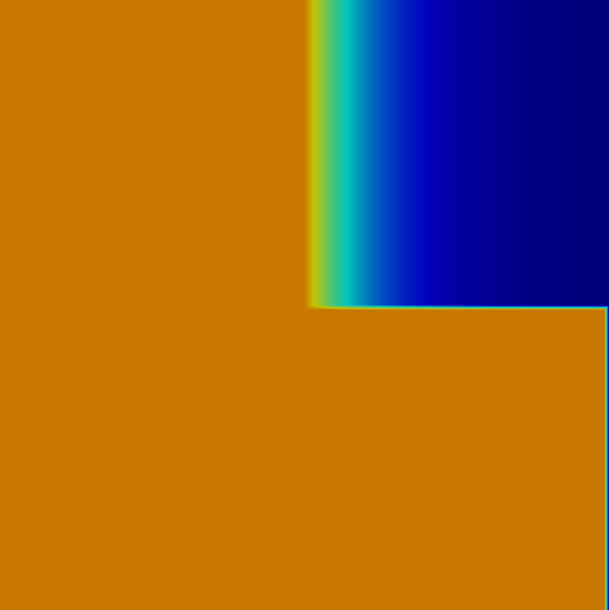
\includegraphics[width=\textwidth]
        {\contentdir/results/transport/void_to_absorber/exact.png}
      \caption{Exact}
   \end{subfigure}
   \begin{subfigure}{0.3\textwidth}
      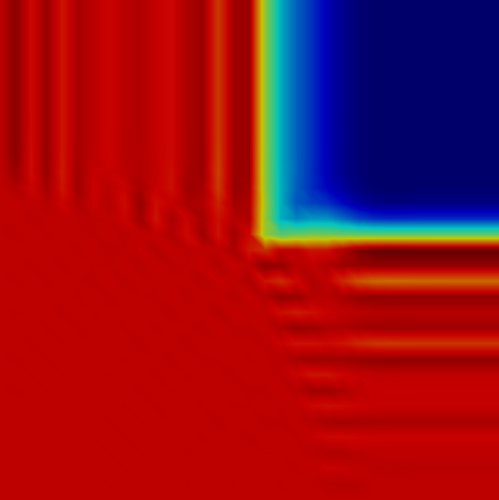
\includegraphics[width=\textwidth]
        {\contentdir/results/transport/void_to_absorber/Gal.png}
      \caption{Galerkin}
   \end{subfigure}
   \begin{subfigure}{0.3\textwidth}
      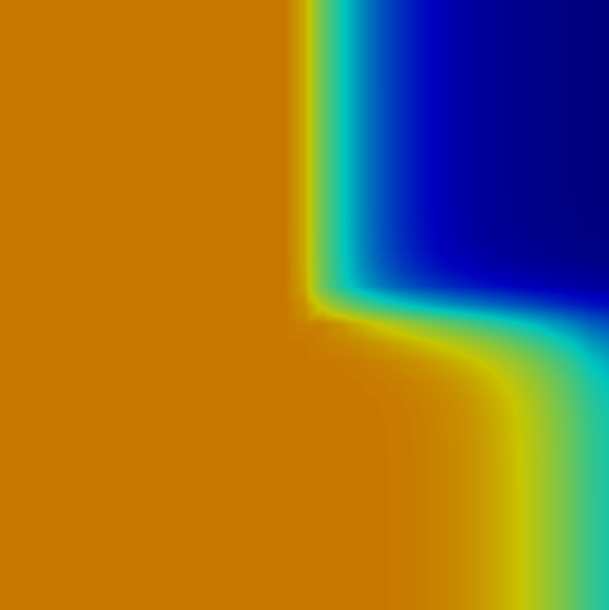
\includegraphics[width=\textwidth]
        {\contentdir/results/transport/void_to_absorber/GalFCT.png}
      \caption{Galerkin with FCT}
   \end{subfigure}
   \begin{subfigure}{0.3\textwidth}
      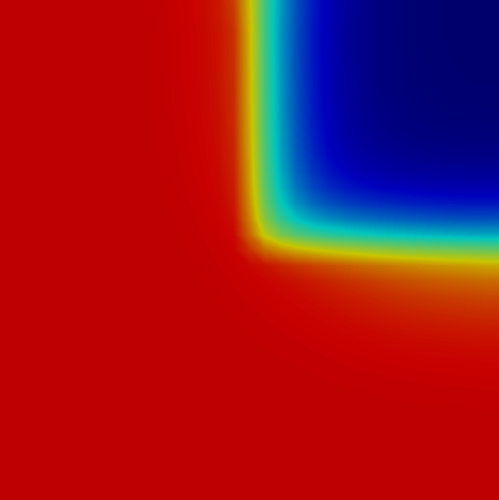
\includegraphics[width=\textwidth]
        {\contentdir/results/transport/void_to_absorber/low.png}
      \caption{Low-order}
   \end{subfigure}
   \begin{subfigure}{0.3\textwidth}
      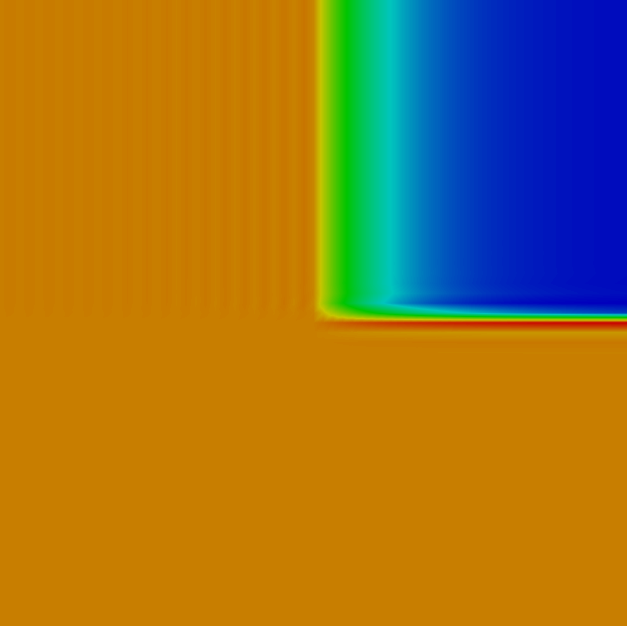
\includegraphics[width=\textwidth]
        {\contentdir/results/transport/void_to_absorber/EV.png}
      \caption{Entropy Viscosity}
   \end{subfigure}
   \begin{subfigure}{0.3\textwidth}
      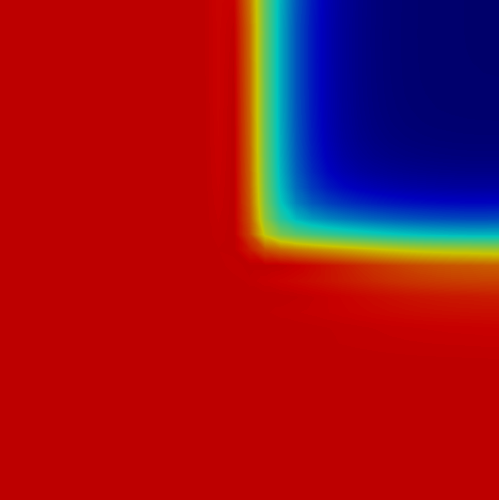
\includegraphics[width=\textwidth]
        {\contentdir/results/transport/void_to_absorber/EVFCT.png}
      \caption{Entropy Viscosity with FCT}
   \end{subfigure}
   \caption{Comparison of Solutions for 2-D Void-to-Absorber Test Problem}
   \label{fig:void_to_absorber_2D}
\end{figure}
%-------------------------------------------------------------------------------
\begin{figure}[ht]
   \centering
   \begin{subfigure}{0.45\textwidth}
      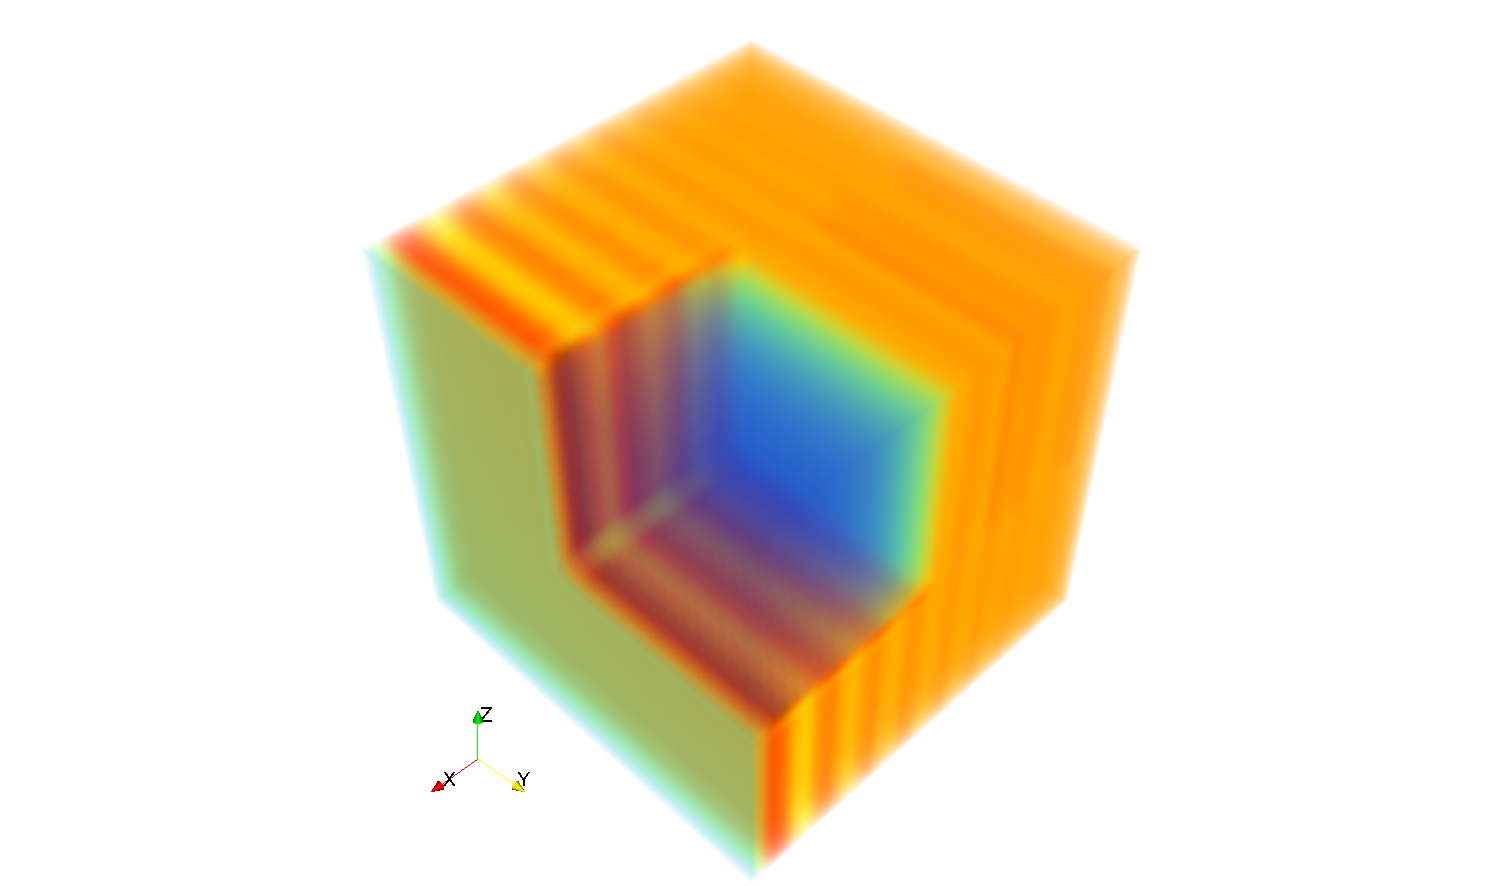
\includegraphics[width=\textwidth]
        {\contentdir/results/transport/void_to_absorber/Gal_3D.png}
      \caption{Galerkin}
   \end{subfigure}
   \begin{subfigure}{0.45\textwidth}
      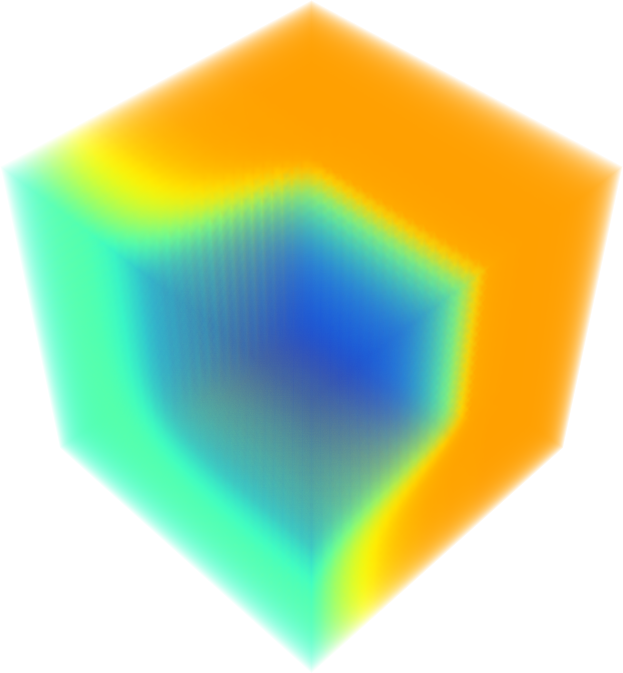
\includegraphics[width=\textwidth]
        {\contentdir/results/transport/void_to_absorber/GalFCT_3D.png}
      \caption{Galerkin with FCT}
   \end{subfigure}
   \caption{Comparison of Solutions for the 3-D Void-to-Absorber Test Problem}
   \label{fig:void_to_absorber_3D}
\end{figure}
%-------------------------------------------------------------------------------
